\documentclass[12pt,a4paper,oneside]{ctexart}

\usepackage{amsmath, amsthm, amssymb, graphicx}
\usepackage[bookmarks=true, colorlinks, citecolor=blue, linkcolor=black]{hyperref}
\usepackage{listings}
\usepackage{xcolor}
\usepackage[export]{adjustbox}
\usepackage{multirow}
\usepackage{makecell}
\usepackage{ulem}
\usepackage{extarrows}
\usepackage{enumitem}
\usepackage{appendix}
\usepackage{subfig}
\usepackage{colortbl}
\usepackage{diagbox}
\usepackage{caption}
\captionsetup[table]{font=small}

% Times New Roman replacement for PDFTeX
\usepackage{mathptmx} % Use Times font
\usepackage{helvet}   % Use Helvetica for sans-serif
\usepackage{courier}  % Use Courier for monospace

% Custom colors for listings
\definecolor{mygray}{RGB}{245,245,245}
\lstset{
	tabsize=4,
	frame=tb,
	commentstyle=\color{red!50!green!50!blue!50},
	rulesepcolor=\color{red!20!green!20!blue!20},
	keywordstyle=\color{blue!90}\bfseries,
	backgroundcolor=\color{mygray},
	showstringspaces=false,
	stringstyle=\ttfamily,
	basicstyle={\footnotesize\ttfamily},
	breaklines=true,
	keepspaces=true,
	lineskip=-0.1pt,
	captionpos=t,
	breakautoindent=true
}

% Table spacing adjustments
\renewcommand{\arraystretch}{1.5}

% Page headers
\usepackage{fancyhdr}
\pagestyle{fancy}
\fancyhf{}
\fancyhead[L]{\songti\zihao{-4}\leftmark}
\fancyhead[R]{\thepage}

\begin{document}

		\begin{titlepage}
			\begin{center}
				\par
				
\includegraphics[width=1\linewidth]{SCUT1}
				\par
				\vskip 1cm
				\fontsize{30}{0}\textbf{VHDL Experimental Report}
				\vskip 3.5cm
				\large
				\begin{table}[!ht]
					\renewcommand{\arraystretch}{2}
					\fontsize{15}{0}
					\heiti
					\begin{tabular}{p{3cm} p{10cm}<{\centering}}
						Curriculum: & Digital System Design (Experiment) \\
						\cline{2-2}
						Student Name: & Liu Xingyan/\fontsize{13}{0}刘兴琰\\
						\cline{2-2}
						Student No.: & \large202264690069 \\
						\cline{2-2}
						Student Major: & Artificial Intelligence/\fontsize{13}{0}人工智能 \\
						\cline{2-2}
						Examiner: & Wu Hancong/\fontsize{13}{0}吴瀚聪\\
						\cline{2-2}
					\end{tabular}
				\end{table}
				\vskip 2cm
				
\includegraphics[width=0.6\linewidth]{FT3.png} 
			\end{center}
		\end{titlepage}

\newpage

\begin{table}[!ht]
	\centering
	\begin{tabular}{|m{3.2cm}|m{3.2cm}|m{3.2cm}|m{3.2cm}|}
		\hline
		\textbf{Name} & 刘兴琰 & \textbf{Class} & 22人工智能1班 \\[0.2cm]
		\hline
		\textbf{Date} & 11月20日 & \textbf{Score} & \\[0.2cm]
		\hline
		\textbf{Examiner} & 吴瀚聪 & & \\[0.2cm]
		\hline
	\end{tabular}
\end{table}

\section{Experiment Procedure}

\subsection{Experiment Purpose}
\begin{itemize}
    \item Learn the basics of VHDL programming.
    \item Practice writing, compiling, and debugging VHDL code in Quartus II.
    \item Test and verify designs through simulations in Quartus II and ModelSim.
\end{itemize}

\subsection{Experiment Tools}
\begin{itemize}
    \item \textbf{Quartus II 13.1 (64-bit)}
    \item \textbf{ModelSim SE-64 10.4}
\end{itemize}

\subsection{Experiment Tasks}
\begin{enumerate}
    \item  Follow the instructions to create a basic 1-bit adder circuit.
    \item  Use the 1-bit adder as a reusable component in a package.
    \item  Combine multiple 1-bit adders to create a 4-bit adder.
    \item  Create a symbol file for the 4-bit adder using Quartus II.
    \item  Test the 4-bit adder by running a waveform simulation.
    \item  Use ModelSim to verify the design and document the outputs.
\end{enumerate}


\subsection{Detailed Procedure}

\subsubsection{Design a 1-bit Adder}
The hardware encapsulation of a 1-bit full adder is shown below:

\begin{figure}[h]
    \centering
    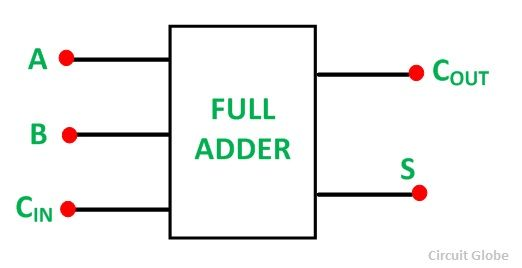
\includegraphics[width=0.6\linewidth]{1.jpg}
    \caption{1-bit Full Adder}
\end{figure}
These equations define the 1-bit full adder for implementation in hardware.
\[
S = A \oplus B \oplus \text{Cin}
\]

\[
\text{Cout} = (A \land B) \lor (A \land \text{Cin}) \lor (B \land \text{Cin})
\]

Expanded forms:

\[
S = (A \lor B \lor \text{Cin}) \land \neg((A \land B) \lor (A \land \text{Cin}) \lor (B \land \text{Cin}))
\]

\[
\text{Cout} = (A \land B) \lor (\text{Cin} \land (A \lor B))
\]

Write the following VHDL code after creating a Quartus II project:
\begin{lstlisting}[language=VHDL, caption=VHDL Code for 1-bit Full Adder, label=lst:fadd_code]
LIBRARY IEEE;
USE IEEE.std_logic_1164.ALL;

ENTITY fadd IS
PORT (a, b, ci: IN std_logic;
      co, sum: OUT std_logic
     );
END fadd;

architecture dataflow of fadd is
begin
    co <= (a and b) or (b and ci) or (a and ci);
    sum <= a xor b xor ci;
end dataflow;
\end{lstlisting}
Compile the code by pressing the "Start Compilation" button to ensure functionality.

\subsubsection{Instantiate the 1-bit Adder as a Component}
The 1-bit adder is encapsulated as a reusable component within a package. The package \texttt{components} declares the component \texttt{fadd}, which defines the input ports \texttt{a}, \texttt{b}, and \texttt{ci}, and the output ports \texttt{co} and \texttt{sum}. This allows the 1-bit adder to be instantiated multiple times in hierarchical designs. The VHDL code for the component declaration is shown below:

\begin{lstlisting}[language=VHDL, caption=VHDL Code for Component Declaration, label=lst:component_declaration]
LIBRARY IEEE;
USE IEEE.std_logic_1164.ALL;

package components is
    component fadd is
        port (
            a, b, ci: IN std_logic;
            co, sum: OUT std_logic
        );
    end component;
end components;
\end{lstlisting}

\subsubsection{Design a 4-bit Adder Using the 1-bit Adder Component}
Using the 1-bit adder component declared in the package, a 4-bit adder is designed by instantiating four instances of the 1-bit adder. The entity \texttt{fadd4} defines the inputs \texttt{a} and \texttt{b} as 4-bit vectors, the carry-in (\texttt{ci}), and the outputs \texttt{sum} (a 4-bit vector) and \texttt{co} (carry-out). The architecture \texttt{stru} of the 4-bit adder connects the four 1-bit adders sequentially, with the carry-out signal of each stage passed to the carry-in signal of the next stage via an internal signal \texttt{ci\_ns}. The complete VHDL code for the 4-bit adder is shown below:

\begin{lstlisting}[language=VHDL, caption=VHDL Code for 4-bit Adder, label=lst:fadd4_code]
USE IEEE.std_logic_1164.ALL;
USE work.components.all;

entity fadd4 is
port (
    a, b: in std_logic_vector(3 downto 0);
    ci: in std_logic;
    co: out std_logic;
    sum: out std_logic_vector(3 downto 0)
);
end fadd4;

ARCHITECTURE stru OF fadd4 IS
SIGNAL ci_ns: std_logic_vector(2 downto 0);
BEGIN
    U0: fadd PORT MAP (
        a => a(0),
        b => b(0),
        ci => ci,
        co => ci_ns(0),
        sum => sum(0)
    );
    U1: fadd PORT MAP (
        a => a(1),
        b => b(1),
        ci => ci_ns(0),
        co => ci_ns(1),
        sum => sum(1)
    );
    U2: fadd PORT MAP (
        a => a(2),
        b => b(2),
        ci => ci_ns(1),
        co => ci_ns(2),
        sum => sum(2)
    );
    U3: fadd PORT MAP (
        a => a(3),
        b => b(3),
        ci => ci_ns(2),
        co => co,
        sum => sum(3)
    );
END stru;
\end{lstlisting}


\subsubsection{Create a Symbol File of the 4-bit Adder and Check It}

The symbols for the 4-bit adder (\texttt{adder\_4bit}) and 1-bit adder (\texttt{adder\_1bit}) were generated using Quartus II. These symbols allow for graphical representation and integration of the respective modules in schematic designs. The updated symbols are shown below:

\begin{figure}[h]
    \centering
    \subfloat[Symbol of \texttt{adder\_4bit}]{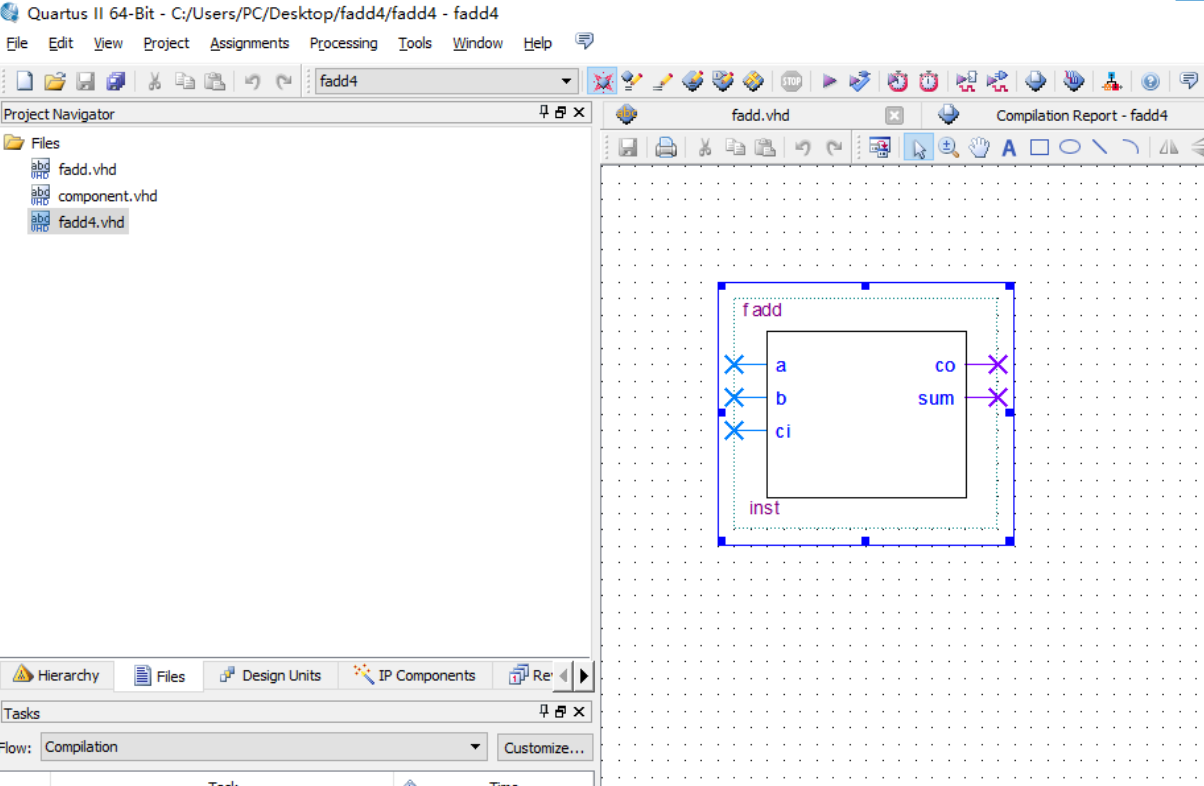
\includegraphics[width=0.4\linewidth]{symbol_adder4bit}} 
    \subfloat[Symbol of \texttt{adder\_1bit}]{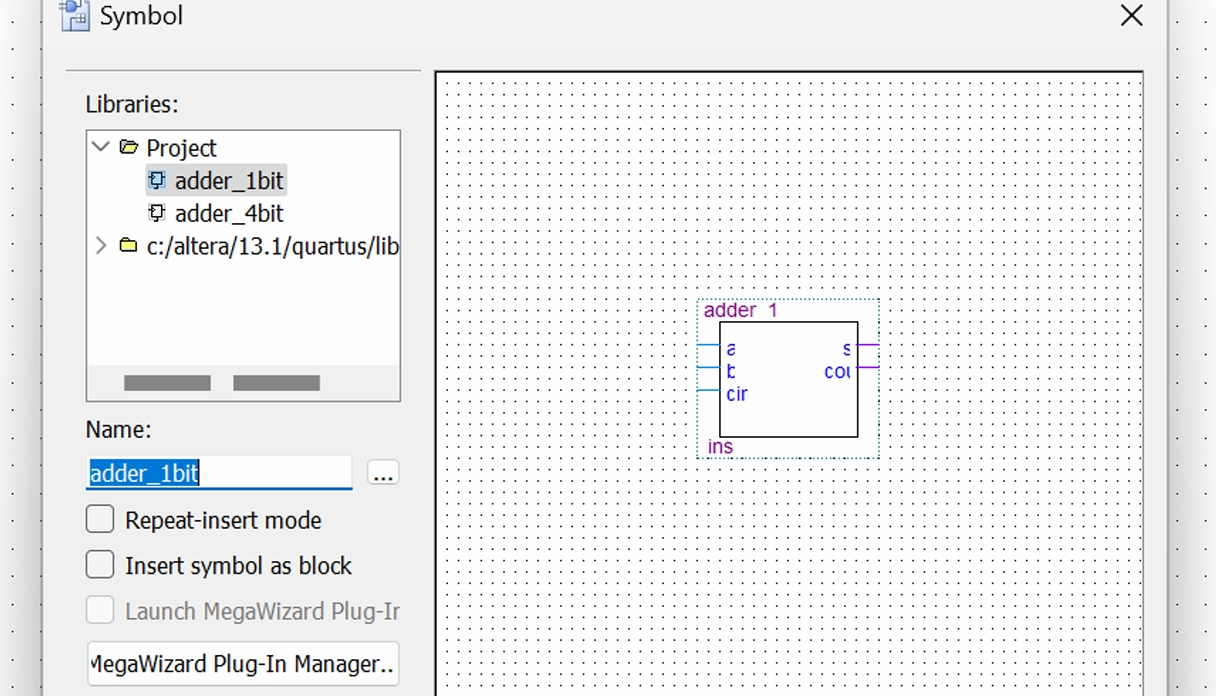
\includegraphics[width=0.4\linewidth]{symbol_adder1bit}} 
    \caption{Symbols of \texttt{adder\_4bit} and \texttt{adder\_1bit}}
    \label{fig:symbols}
\end{figure}

\subsubsection{Perform Waveform Simulation and Record Results}

To validate the functionality of the 4-bit adder, a testbench was created in ModelSim to perform waveform simulation. The architecture \texttt{fadd4\_arch} includes the declaration of internal signals for the inputs (\texttt{a}, \texttt{b}, \texttt{ci}), the outputs (\texttt{sum}, \texttt{co}), and connections between the master ports and the adder component.

The testbench initializes the inputs as follows:
\begin{itemize}
    \item \texttt{a} = \texttt{"0000"}
    \item \texttt{b} = \texttt{"0000"}
    \item \texttt{ci} = \texttt{'0'}
\end{itemize}

The key testbench code snippet is shown below:

\begin{lstlisting}[language=VHDL, caption=Testbench Code for 4-bit Adder Simulation]
ARCHITECTURE fadd4_arch OF fadd4_vhd_tst IS
    -- Constants
    SIGNAL a : STD_LOGIC_VECTOR(3 DOWNTO 0);
    SIGNAL b : STD_LOGIC_VECTOR(3 DOWNTO 0);
    SIGNAL ci : STD_LOGIC;
    SIGNAL co : STD_LOGIC;
    SIGNAL sum : STD_LOGIC_VECTOR(3 DOWNTO 0);

BEGIN
    U1: fadd4 PORT MAP (
        a => a,
        b => b,
        ci => ci,
        co => co,
        sum => sum
    );

    init : PROCESS
    BEGIN
        a <= "0000";
        b <= "0000";
        ci <= '0';
        FOR k IN 0 TO 1 LOOP
            FOR j IN 0 TO 3 LOOP
                FOR i IN 0 TO 3 LOOP
                    WAIT FOR 10 ns;
                    a <= a + 1;
                END LOOP;
                b <= b + 1;
            END LOOP;
            ci <= NOT ci;
        END LOOP;
        WAIT;
    END PROCESS init;
END fadd4_arch;
\end{lstlisting}

A nested loop iterates through all possible combinations of the 4-bit inputs \texttt{a} and \texttt{b} with the carry-in signal toggled for each complete iteration. At each step:
\begin{itemize}
    \item The inputs \texttt{a} and \texttt{b} are incremented sequentially.
    \item A delay of \texttt{10 ns} is added between transitions.
    \item The carry-in signal \texttt{ci} is toggled after each full sequence.
\end{itemize}

The connections to the instantiated \texttt{fadd4} component ensure the correct mapping of inputs and outputs for simulation. After running the testbench, the waveform results are generated in ModelSim, verifying the correct behavior of the 4-bit adder.

\section{Experimental Record}

\begin{enumerate}
    \item \textbf{Design Code of the Adders:}
    \begin{itemize}
        \item (a) \texttt{adder\_1bit}
        \begin{figure}[h]
            \centering
            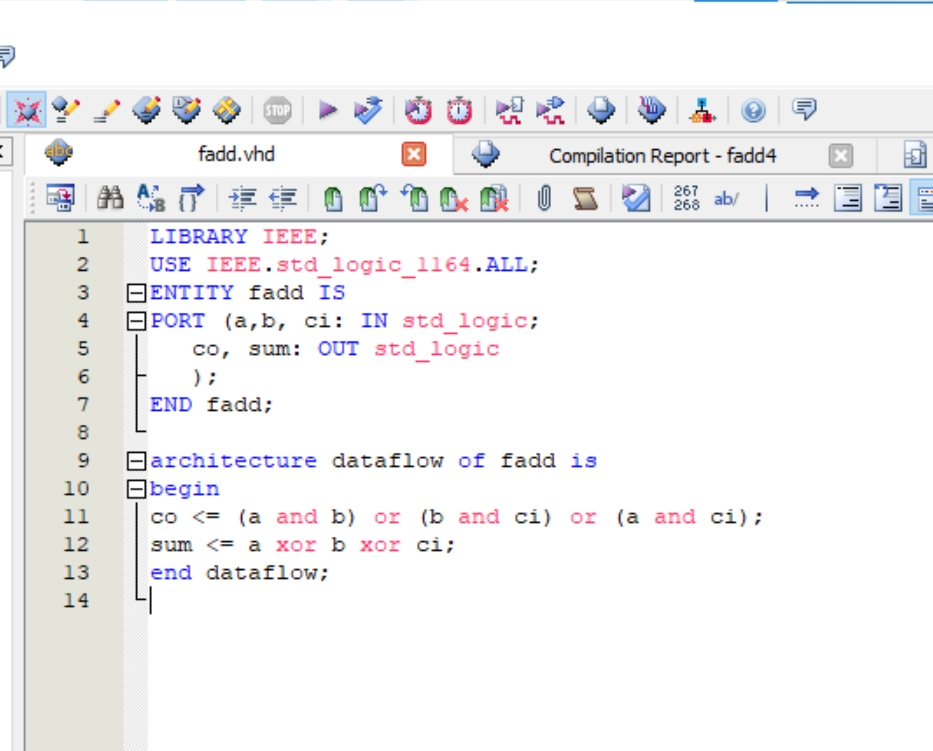
\includegraphics[width=0.4\linewidth]{adder_1bit_code} % Replace with actual filename
            \caption{Design Code of \texttt{adder\_1bit}}
            \label{fig:adder_1bit_code}
        \end{figure}
        \item (b) \texttt{adder\_4bit}
        \begin{figure}[h]
            \centering
            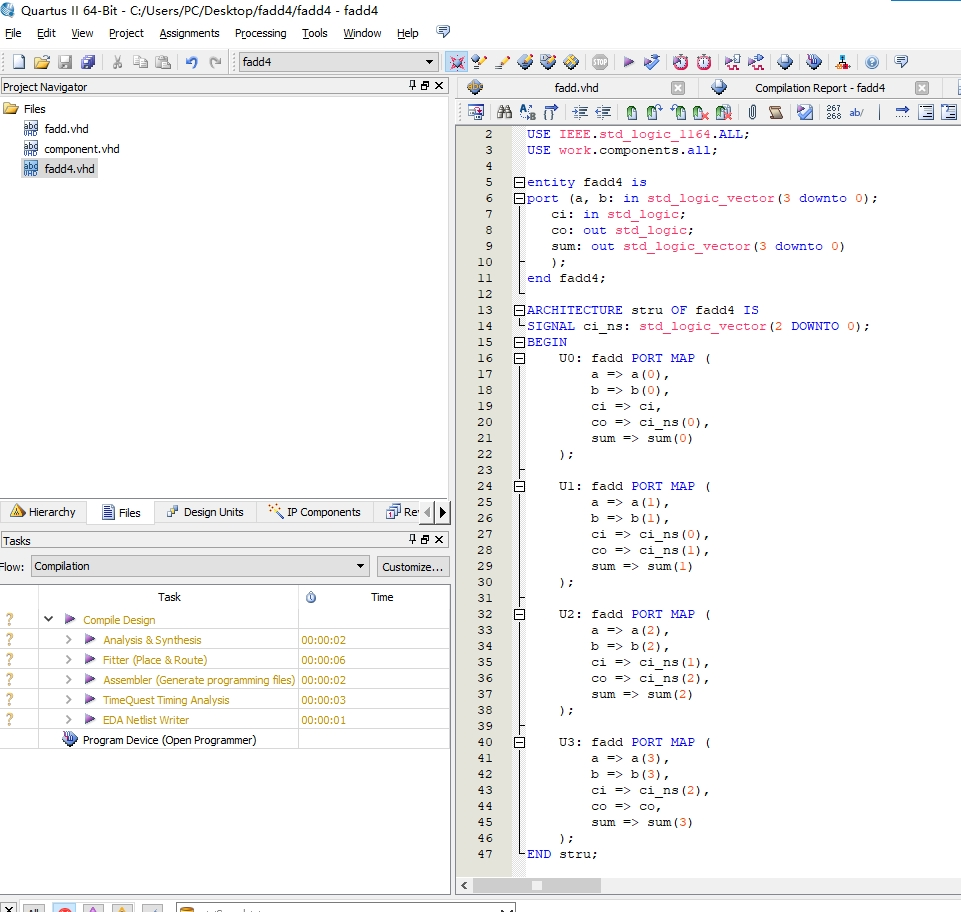
\includegraphics[width=0.65\linewidth]{adder_4bit_code} % Replace with actual filename
            \caption{Design Code of \texttt{adder\_4bit}}
            \label{fig:adder_4bit_code}
        \end{figure}
    \end{itemize}

\section{Analysis and Discussion}

The simulation results confirm that the 4-bit adder functions correctly. It adds the inputs from ports \texttt{a} and \texttt{b} and outputs the sum through port \texttt{s}. The carry-out signal at port \texttt{cout} correctly indicates overflow.

Minor glitches caused by signal delays or hazards were observed but did not impact the adder’s functionality. The design meets all operational requirements under simulation.


\section{Other Attachments}

\begin{itemize}
    \item \textbf{Waveform of \texttt{adder\_4bit}:}
    \begin{itemize}
        \item (a) Waveform 1
        \begin{figure}[h]
            \centering
            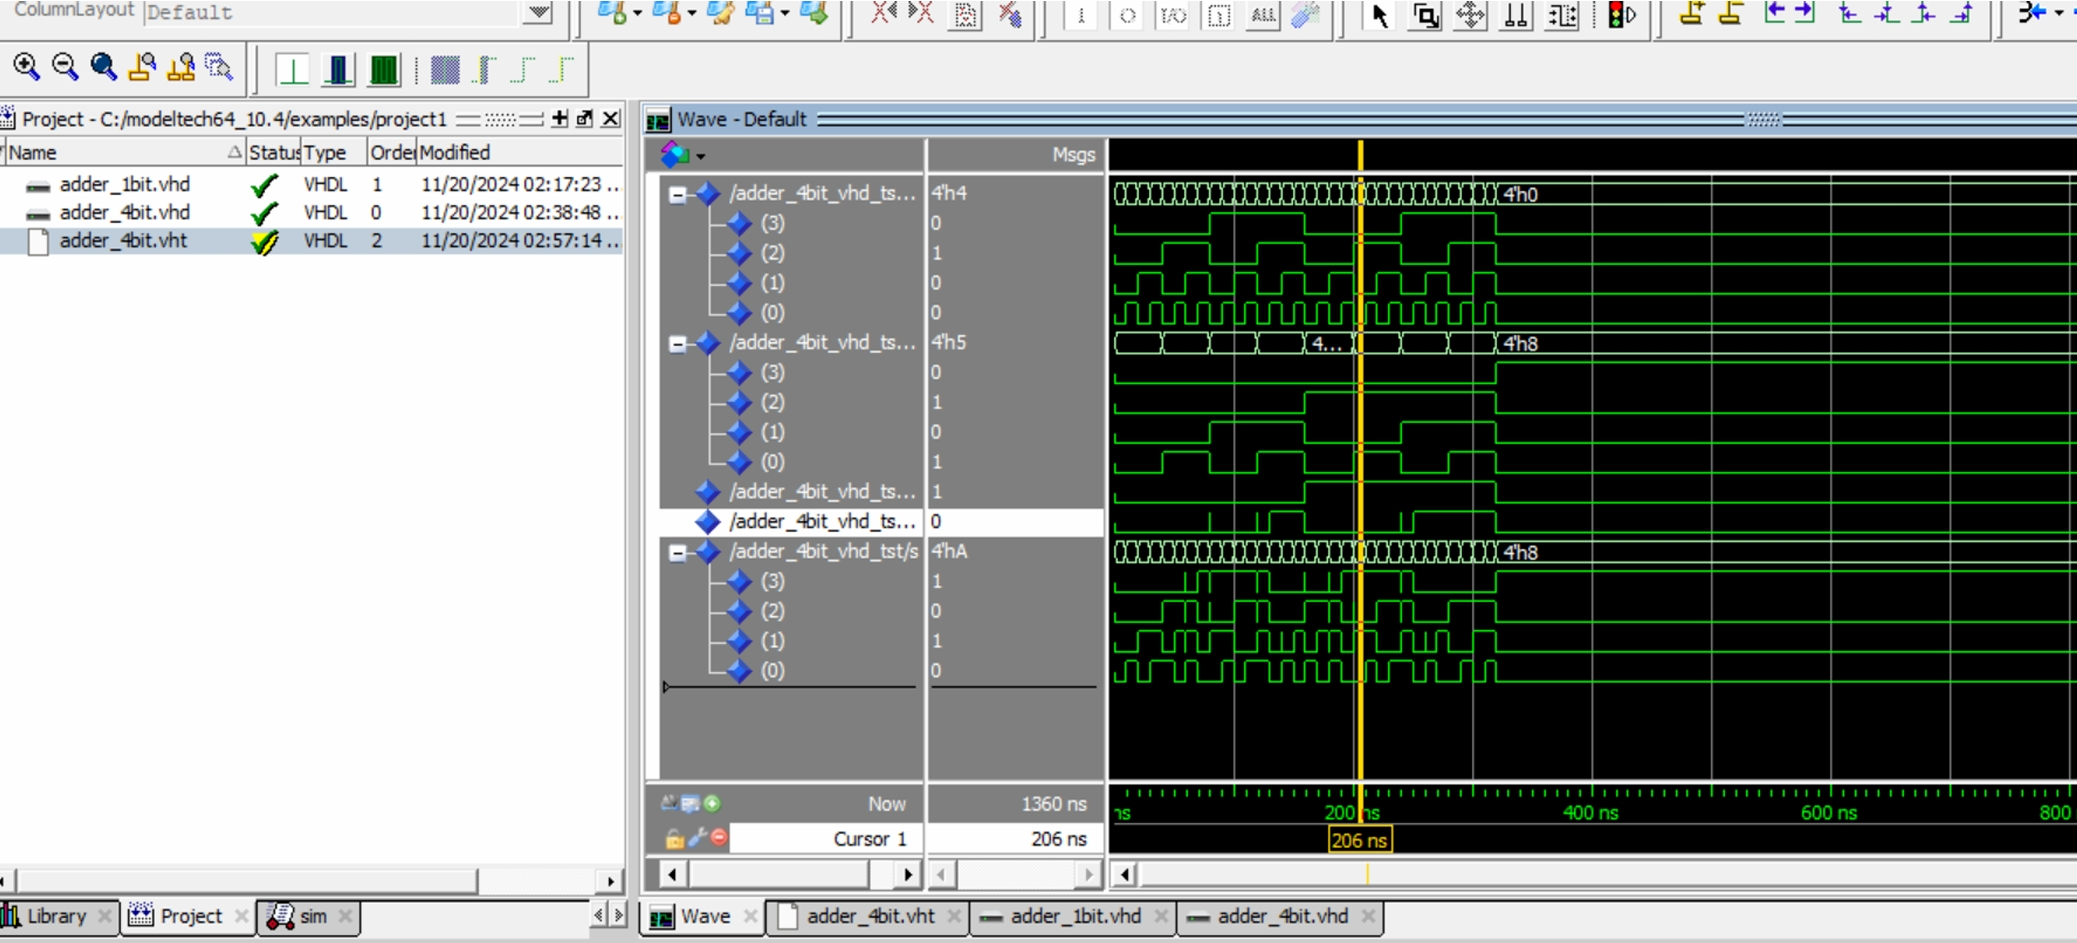
\includegraphics[width=0.6\linewidth]{waveform_1} % Replace with actual filename
            \caption{Waveform 1 of \texttt{adder\_4bit}}
            \label{fig:waveform_1}
        \end{figure}
        \item (b) Waveform 2
        \begin{figure}[h]
            \centering
            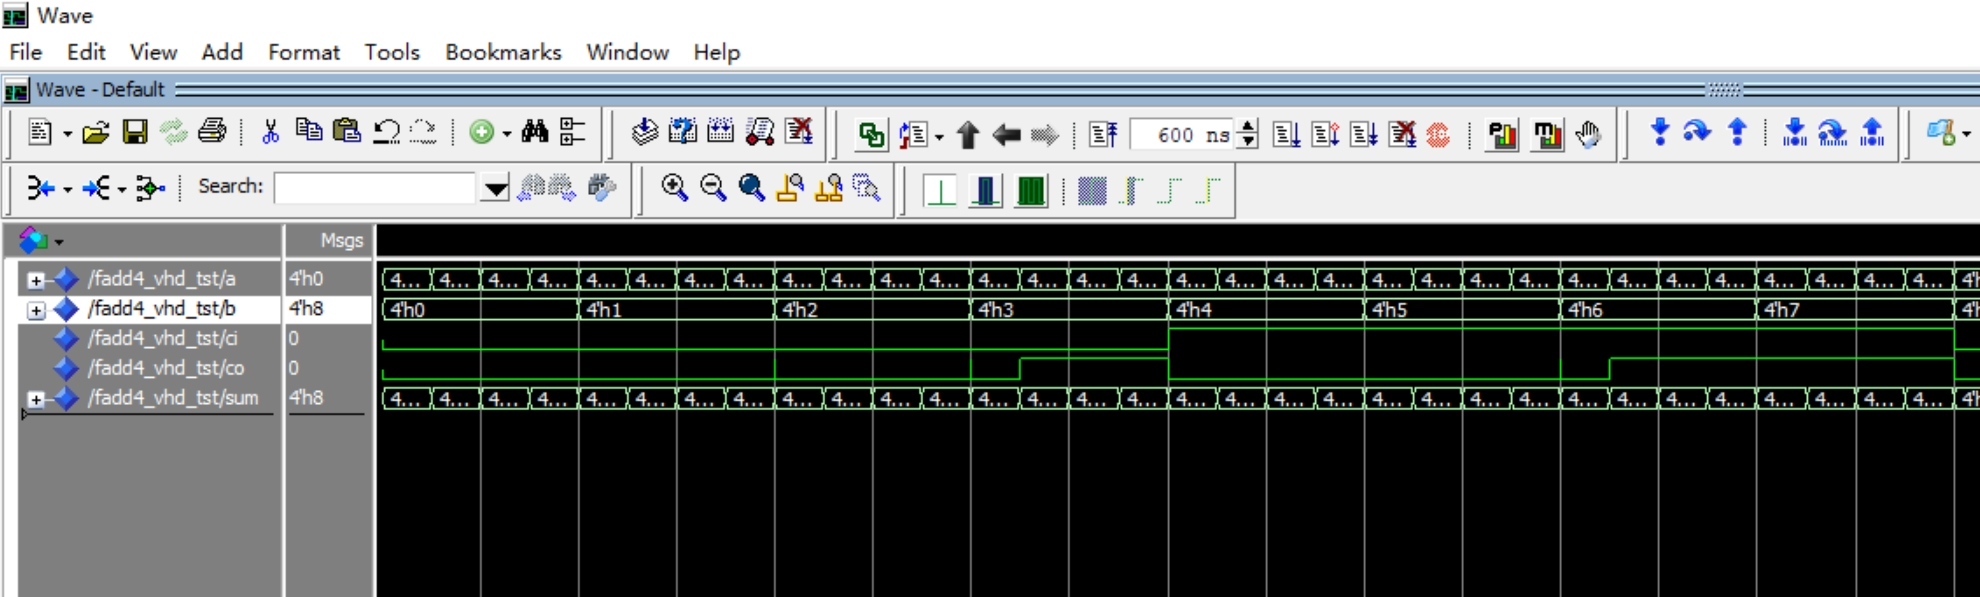
\includegraphics[width=0.6\linewidth]{waveform_2} % Replace with actual filename
            \caption{Waveform 2 of \texttt{adder\_4bit}}
            \label{fig:waveform_2}
        \end{figure}
    \end{itemize}
\end{itemize}


\end{document}
